\documentclass[border=10pt]{standalone}
\usepackage{tikz}
\usetikzlibrary{positioning,arrows.meta,calc,fit,patterns}

\begin{document}
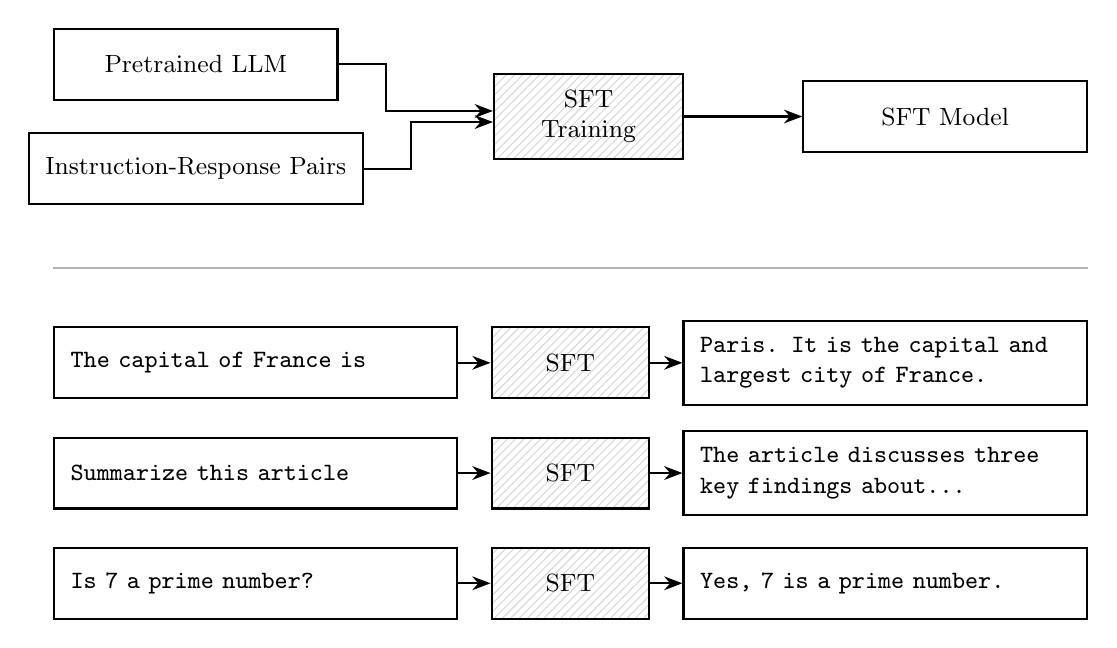
\begin{tikzpicture}[
    >=Stealth,
    every node/.style={font=\small},
    box/.style={draw, thick, minimum height=0.9cm, inner sep=6pt, text centered},
    inputbox/.style={box, fill=white, align=left},
    outputbox/.style={box, fill=white, align=left},
    modelbox/.style={box, pattern=north east lines, pattern color=black!15, minimum width=2.0cm, minimum height=0.9cm, align=center},
    flowbox/.style={box, fill=white, minimum width=3.6cm},
    flowarrow/.style={->, thick, black},
]

% ---- Top: Process Flow ----
\node[flowbox] (pretrained) {Pretrained LLM};
\node[flowbox, below=0.4cm of pretrained] (data) {Instruction-Response Pairs};
\node[modelbox, right=1.8cm of $(pretrained.east)!0.5!(data.east)$, minimum width=2.4cm] (sft) {SFT\\Training};
\node[flowbox, right=1.5cm of sft] (sftmodel) {SFT Model};

% Arrows from both inputs enter SFT at different heights
\draw[flowarrow] (pretrained.east) -- ++(0.6cm,0) |- ([yshift=2pt]sft.west);
\draw[flowarrow] (data.east) -- ++(0.6cm,0) |- ([yshift=-2pt]sft.west);
\draw[flowarrow] (sft) -- (sftmodel);

% ---- Divider ----
\coordinate (leftedge) at (pretrained.west);
\coordinate (rightedge) at (sftmodel.east);
\draw[thick, black!30] ([yshift=-0.8cm]leftedge |- data.south) -- ([yshift=-0.8cm]rightedge |- data.south);

% ---- Bottom: Example I/O (centered, equal widths) ----
\coordinate (figcenter) at ($(leftedge)!0.5!(rightedge)$);

\coordinate (row1) at ([yshift=-2.0cm]data.south -| figcenter);
\coordinate (row2) at ([yshift=-1.4cm]row1);
\coordinate (row3) at ([yshift=-1.4cm]row2);

% Place model boxes at the true center
\node[modelbox, minimum width=2.0cm] (m1) at (row1) {SFT};
\node[modelbox, minimum width=2.0cm] (m2) at (row2) {SFT};
\node[modelbox, minimum width=2.0cm] (m3) at (row3) {SFT};

% Row 1
\node[inputbox, text width=4.7cm, anchor=west] (in1) at (leftedge |- row1) {\texttt{The capital of France is}};
\node[outputbox, text width=4.7cm, anchor=east] (out1) at (rightedge |- row1) {\texttt{Paris. It is the capital and largest city of France.}};
\draw[flowarrow] (in1) -- (m1);
\draw[flowarrow] (m1) -- (out1);

% Row 2
\node[inputbox, text width=4.7cm, anchor=west] (in2) at (leftedge |- row2) {\texttt{Summarize this article}};
\node[outputbox, text width=4.7cm, anchor=east] (out2) at (rightedge |- row2) {\texttt{The article discusses three key findings about...}};
\draw[flowarrow] (in2) -- (m2);
\draw[flowarrow] (m2) -- (out2);

% Row 3
\node[inputbox, text width=4.7cm, anchor=west] (in3) at (leftedge |- row3) {\texttt{Is 7 a prime number?}};
\node[outputbox, text width=4.7cm, anchor=east] (out3) at (rightedge |- row3) {\texttt{Yes, 7 is a prime number.}};
\draw[flowarrow] (in3) -- (m3);
\draw[flowarrow] (m3) -- (out3);

\end{tikzpicture}
\end{document}
